\section{Single Photon Avalanche Detector}
	\label{SPAD}

	
	\subsection{Avalanche Diodes}
		\label{diodes}
		
Essentially, a \ac{SPAD} is a reversed biased \textit{p-n junction} that operates at a voltage level above the breakdown voltage. At this bias, the electric field is so high that a single charge carrier injected into the depletion layer can trigger a self-sustaining avalanche. The current rises swiftly (nanoseconds or subnanosecond rise time) to a macroscopic steady level in the milliampere range. Bias supply voltage Va exceeds breakdown voltage (non-destructive and reversible process) $V_b$ by an amount called the \textit{excess bias voltage} $V_e = (V_a - V_b)$, which has a determining influence on detector performance. Actually, the value of the ratio $V_e/V_b$ is important, not the value of $V_e$ alone, because the performance is related to the excess electric field above breakdown level.  

If the primary carrier is photogenerated, the leading edge of the avalanche pulse marks the arrival time of the detected photon. The current continues to flow until the avalanche can be quenched by lowering the bias voltage to the breakdown voltage ($V_b$) or below. For a photon to be detected, not only must it be absorbed in the detector active volume and generate a primary carrier (more precisely, an electron-hole pair, i.e. \textit{an exciton}), it is also necessary that the primary carrier succeeds in triggering an avalanche. The efficiency of photon detection thus increases with excess bias voltage $V_e$, since higher electric field gradient enhances the triggering probability.   

As it happens in \acp{PMT}, thermal generation effects produce current pulses even in the absence of illumination, and the Poissonian fluctuation of the dark counts represents the internal noise source of the detector. \textit{Dark-count rate} includes primary and secondary pulses. \textit{Primary dark pulses} are due to carriers thermally generated in the \acs{SPAD} junction, so that the count rate increases with the temperature as does the dark current in ordinary photodiodes. The rate also increases with $V_e$ because of field-assisted enhancement of the emission rate from generation centers and an increase in triggering probability. \textit{Secondary dark pulses} are due to afterpulsing effects that may strongly enhance the total dark-count rate. During avalanche some carriers are captured by deep levels in the junction depletion layer and subsequently released with a statistically fluctuating delay. Released carriers can retrigger the avalanche, generating afterpulses correlated with a previous avalanche pulse. The number of carriers captured during the avalanche pulse increases with the total number of carriers crossing the junction, that is, with the total charge of the avalanche pulse. Therefore afterpulsing increases with the delay of avalanche quenching and the current intensity, which is proportional to excess bias voltage $V_e$.

\begin{figure} [ht]
	\begin{center}
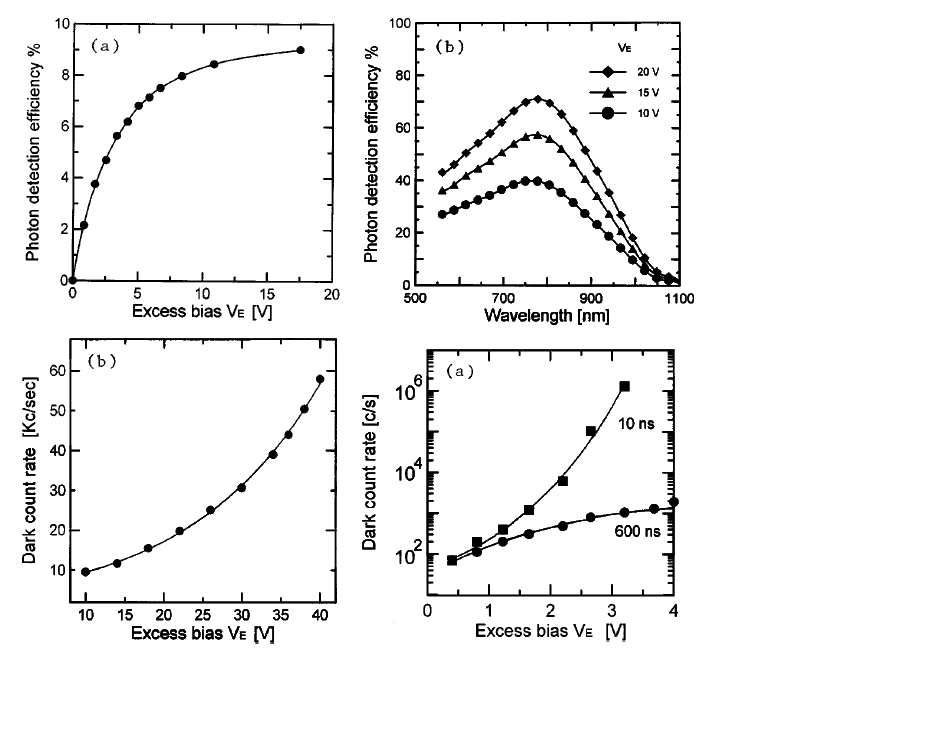
\includegraphics[scale=0.5]{chapters/img/SPAD_Ve_functions.png}	
\caption{}
\label{spad}
\end{center}
\end{figure}

	\subsection{Quenching Circuits}
		\label{AQC}
The bias voltage is then restored, in order to be able to detect another photon. 	
 